\documentclass[12pt,a4paper]{article}
\usepackage[hyperref]{acl2020}
\usepackage{times}
\usepackage{amsmath}
\usepackage{graphicx}
\usepackage{tabularx}
\usepackage{amsfonts}
\usepackage{booktabs}
\usepackage{float}
\usepackage{enumitem}
\usepackage{latexsym}
\usepackage{natbib}
\usepackage[activate={true,nocompatibility},final,tracking=true,kerning=true,spacing=true,factor=1100,stretch=10,shrink=10]{microtype}

\graphicspath{{./images}}
\bibliographystyle{unsrtnat}

\pagestyle{plain}

\aclfinalcopy % Uncomment this line for the final submission
\def\aclpaperid{***} %  Enter the acl Paper ID here

%\setlength\titlebox{5cm}
% You can expand the titlebox if you need extra space
% to show all the authors. Please do not make the titlebox
% smaller than 5cm (the original size); we will check this
% in the camera-ready version and ask you to change it back.

\title{Assessing Word embedding Performance in Multi-Domain Dialogue State Tracking}

\author{Sanchit Nevgi \\
  College of Information and Computer Sciences \\ University of Massachusetts, Amherst}

\date{\today}

\begin{document}
\maketitle

\begin{abstract}
  Recent advancements have made Task-oriented dialogue systems easily accessible, by reducing reliance on hand-crafted features. Dialogue State Tracking is a core component of these systems. Traditional approaches fall short in tracking unknown slot values and cannot easily adapt to new, unseen domains. Recent efforts in dialogue state tracking have progressed towards open vocabulary and generation-based approaches, where the models can generate slot values from the dialogue history itself. In this paper, we assess the quality of various word embeddings when used in the utterance encoder of a task-oriented system. Our results show that pre-trained word vectors perform better in the zero-shot approach.
\end{abstract}

\section{Introduction}

Advancements in neural architectures \cite{Vaswani2017AttentionIA, Devlin2019BERTPO} have led to improvements in dialogue systems A dialogue system is an entity you can interface with via text/voice that has certain capabilities. These capabilities can be broadly classified into three groups \cite{Gao2019NeuralAT}.

\begin{itemize}[leftmargin=0pt, label={}]
  \item \textbf{Question Answering}: QA agents allow users to query large-scale Knowlege Bases (KB-QA) or document collection in natural lanaguage (text-QA). In the real-world, text-QA agents are most commonly used in search engines such as Google, Bing, while KB-QA are widely used in voice assistants.
  \item \textbf{Task-oriented systems}: Task-oriented systems work towads a well-specified goal, such as movie ticket booking, usually in a multi-turn fashion. The dialogue system keeps track of the dialogue state, uses information supplied by user to constrain search, prompts user for required information necessary task completion.
  \item \textbf{Social chatbots}: The agent needs to converse seamlessly with users, provide useful recommendations. A good dialogue agent should demonstrate emotional connect with the user. For example, showing excitement when user shares good news, empathy when user is feeling sad, etc.
\end{itemize}

A dialogue system consists for 4 components ---

\begin{enumerate}
  \setlength\itemsep{0pt}
  \item Natural Language Understanding
  \item Dialogue State Tracking
  \item Dialogue Policy
  \item Natural Language Generation
\end{enumerate}

Dialogue state tracking (DST) is a core component in task-oriented dialogue systems. The goal of DST module is to extract user goals/intentions expressed during conversation and to encode them as a compact set of dialogue states, i.e., a set of slots and their corresponding values \cite{WuTradeDST2019}. Traditionally DST modules used a fixed ontology, where the slot-values were known prior. The task was framed as as a classification problem. However, these models do not scale well and are unable to handle unseen domains. Recent approaches follow a generation approach to handle Out Of Vocabulary terms.

\section{Definitions}

\textbf{Ontology}: An ontology defines the domain of a task-oriented system. It is a structured representation of an external database. The ontology defines all entity attributes called \textit{slots} and all the possible \textit{values} for each slot. In practice, a full ontology is difficult to obtain in advance. Some slots such as dates, names are unbounded. Slots are classified as \textit{Informable} and \textit{Requestable} slots. An \textit{informable} slot (area, price-range) allows the user to constrain the search query, while \textit{requestable} slots (phone-number, operational-time) represent additional information that a user can request from the dialogue system.

\medskip \noindent \textbf{Dialogue Act}: The semantic representation of each turn of a dialogue is known as a \textit{dialogue act}. A dialogue act has an implicit \textit{intent}, \textit{slot-value} pairs or both.

\medskip \noindent \textbf{Slot-filling dialogues}: The user and the system converse with the goal of \textit{slot-filling}. The system must collect all the necessary information from the user to formulate an appropriate query. In the movie ticket booking domain, some examples of slots are \texttt{movie-name, time, price, location}. Slots are \textit{informable} if the user can provide the \textit{slot-value}, used to constrain the search; or slots are \textit{requestable}, where the user can ask the value of the slot from the system (eg \texttt{phone\_number})

\medskip \noindent \textbf{Knowledge Base}: A Knowledge Base (KB) is a structured database conisiting of facts in the form of subject-predicate-object triples $(s, r, t)$, where $s, t \in \mathcal{E}$ are entities and $r \in \mathcal{R}$ are predicates or relations.

\begin{figure}[!ht]
  \centering
  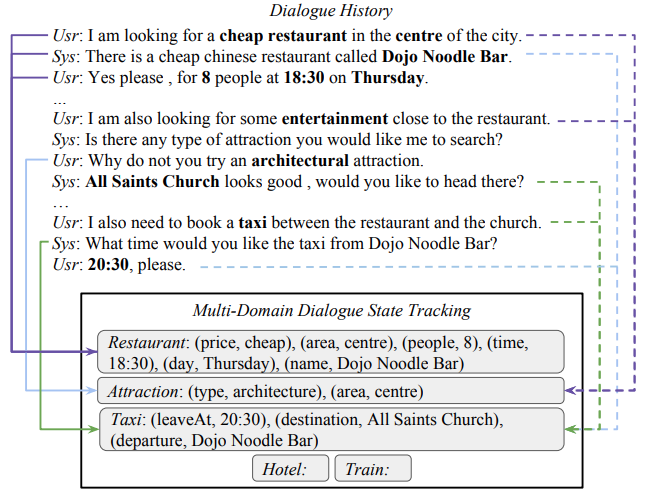
\includegraphics[width=0.5\textwidth]{./images/dst.png}
  \caption{Sample dialogues and corresponding Dialogue State Tracking}
\end{figure}

\section{Related Work}

Learning task-oriented dialogs end-to-end requires defining a user simulator and a dialogue agent. \citeauthor{Bordes2016LearningEG} define baseline tasks to measure neural methods's performances. Traditional dialog systems in task-oriented dialogs require lot of domain-specific handcrafting, which makes it difficult to scale. These limitations are mitigated in end-to-end trained systems. \cite{Bordes2016LearningEG} shows that, compared to hand-crafted slot-filling baseline, end-to-end dialog system based on \textit{Memory networks} \cite{Sukhbaatar2015EndToEndMN} can reach promising, but imperfect performance and can even perform non-trivial operations.

Successful goal-oriented dialog systems model coversation as partially observable Markov deicsion processes. Require hand-crafted features for state and action space representations, restricting to narrow domains. To measure the performance of task-oriented dialog systems, 5 common tasks have been proposed. They are,

\begin{itemize}[leftmargin=*,label={}]
  \setlength\itemsep{0em}
  \item Task 1 - Issuing API calls
  \item Task 2 - Updating API calls
  \item Task 3 - Displaying options
  \item Task 4 - Providing extra information
  \item Task 5 - Full dialogs
\end{itemize}

In \cite{Bordes2016LearningEG}, the authors use a restaurant KB, which has \texttt{name, cuisine, location, price range, address, phone number}. Each example in the dataset comprises of dialog utterances from user and bot, as well as API calls and the resulting facts. They split the KB into two, disjoint sets of \textit{cuisines}, and \textit{locations}, to test the models capability to handle Out-of-Vocabulary scenario. The dialog systems are evaluated in a ranking, not a generation setting. At each turn of dialog, they test whether they can predict bot utterances by selecting candidates.

Further, the model is evaluated on real concierge service where the dialogs are shorter, and the vocabulary more diverse. Some of the findings are that the set of user requests is much wider compared to dataset, from managing restaurant reservation to asking for recommendations. Also, the users do not stay focused on the request. The facts about restaurants are not structured like KB and finally the users and operators make typos, spelling and grammatical erros. Some approaches to modeling task-oriented systems are outlined below,

\begin{enumerate}
  \item Rule-based systems - Use hand-crafted rules such as word matches, positions in dialog, entity detections, dialog state.
  \item Information Retrieval models: Use a TF-IDF matching for each possible candidate response, compute the matching score between input and response. The score is computed as a TF-IDF weighted cosine similarity between the bag-of-words of input and response.
  \item Nearest neighbour - Finds the most similar conversation in the training set and use that response. Word overlap as scoring method. Sorted by decreasing co-occurence frequency.
  \item Supervised embedding models - Predict next response given the previous conversation. Scored for input $x$ as $f(x, y) = (Ax)^TBy$. Trained with margin ranking loss
  \item Memory Networks - We know that ssing word embeddings fails when the dialogue has open-ended entities, since embeddings use approximate word match. They cannot handle OOV words. The solution is to match type features and augment vocabulary with 7 words (cuisine, location, etc).
\end{enumerate}

\medskip \noindent \textbf{Neural Belief Tracker}: \citeauthor{Mrksic2016NeuralBT} proposes an end-to-end trained DST module known at the \textit{Neural Belief Tracker}. A \textit{belief tracker}, estimates the user's goal at every step of the dialog. They mitigate two issues with traditional approaches to building DST, namely that NLU models require large amount of training data and hand-crafting lexicons for capturing liguistic variation in users's language is cumbersome.

Using recent advances in \textit{representation learning}, Neural Belief Tracking (NBT) framework reasons over pre-trained word vectors, learning to compose them into distributed representations of user utterances and dialogue context. The \textit{dialogue state tracking} component serves to interpret user input and update the \textit{belief state}, which is the system's internal representation of teh state of the conversation. The dialogue system is supported by \textit{domain ontology}, which describes the range of user intents the system can process. The ontology defines a collection of slots and the values each slot can take.

The task is non-trivial due to lexical variation, dynamics of context and noisy Automated Speech Recognition (ASR) output. Traditional approaches use separate modules to handle lexical variability in single dialogue turn. However the turn-level SLU and cross-turn DST can be coalesced into a single model, but they rely on manually constructed semantic dictionaries.

Some systems use template-based matching systems while others train independent binary models that decide if slot-value pair was expressed in user utterance. SLU has been treated as sequence labeling problem.

The proposed Neural Belief Tracking model uses pre-trained vectors. The input consists of the system dialogue acts preceding the user input, the user utterance, a single slot-value pair it needs to make a decision about. To perform belief tracking, NBT model iterates over all candidate slot-value pairs and decides which ones have just been expressed by the user. \textit{"I'm looking for good pizza"} entails \textsc{Food=Italian}.

\smallskip \noindent \textbf{Representation Learning module}:
The vector embeddings for unigram, bigram and trigram are concatenated and projected to a fixed-size representation. The canditate slot-value pair and user utterance interact through the \textit{semantic decoding} module. The slot and value representation are concatenated, projected to the same size at user utterance vector and finally a similarity score is computed.

To conclude, the NBT couples Spoken Language Understanding and Dialogue State Tracking without relying on hand-crafted semantic lexicons. Further, the model performance improves with the semantic quality of underlying word vectors.

\medskip \noindent \textbf{Trade DST}: The Trade model \cite{WuTradeDST2019} comprises of three components --- an utterance encoder, a slot gate, and a slot generator. Instead of predicting the probability of every predfined ontology term, the model directly generates the slot values. The utterance encoder encodes the dialogue utterances into a sequence of fixed-length vectors.

The \textit{State Generator} generates slot values using text from the input source using a copy mechanism. \citeauthor{WuTradeDST2019} use a soft-gated pointer generator copy over index-based copying as this helps to extract slot values that are synonyms of values present in the ontology (eg \textit{inexpensive} $\rightarrow$ \textit{cheap}). The decoder uses a GRU to predict the value for each \textit{(domain, slot)} independently. The input to the decoder is a summed vector representation of the domain and slot.

The \textit{Slot gate} is a three-way classifier that maps the dialogue history context vector, the current turn vector representation and for each \textit{(domain, slot)} pair, it independently classifies as one of \textit{(not-mentioned, dont-care, ptr)}, where if the \textit{slot} is not mentioned or no preference is specified we ignore it, otherwise we pass the repsentation to the state generator to extract its value.


\medskip \noindent \textbf{Non-Autoregressive DST} Generation based approaches to dialogue state tracking fall short in two ways; (1) they do not allow models to explicitly learn signals across domains and slots to detect potential dependencies among \textit{(domain, slot)} pairs and (2) existing models follow auto-regressive approaches which incur high time cost when the dialogue evolves over multiple domains and multiple turns. \citeauthor{Le2020NonAutoregressiveDS} propose a non-autoregressive framework which factors in potential dependencies among the domain, slot pairs.

The NADST model consists of 3 components, an encoder, a fertility decoder and a state decoder. Like earlier models, the \textit{encoders} encode sequences of dialogue history, delexicalized dialogue
history, and domain and slot tokens into continuous representations. The \textit{fertility decoder} learns potential dependencies between the domain, slots pairs using an attention mechanism. The embedding weights are shared across all three components. The encoders use token-level embedding and positional encoding to encode the input dialogue history and (domain, slot) pairs into continuous representations. The encoded domains and slots are then input to stacked self-attention and feed-forward network to obtain relevant signals across dialogue history and generate a fertility for each domain, slot pair. The predicted fertilities are used to form an input sequence to the state decoder for nonautoregressive decoding. The output from the state decoder is used as a query to attend on this memory and copy tokens from the dialogue history to generate a dialogue state.

\begin{figure*}[!ht]
  \centering
  \caption{MultiWOZ dataset statistics}
  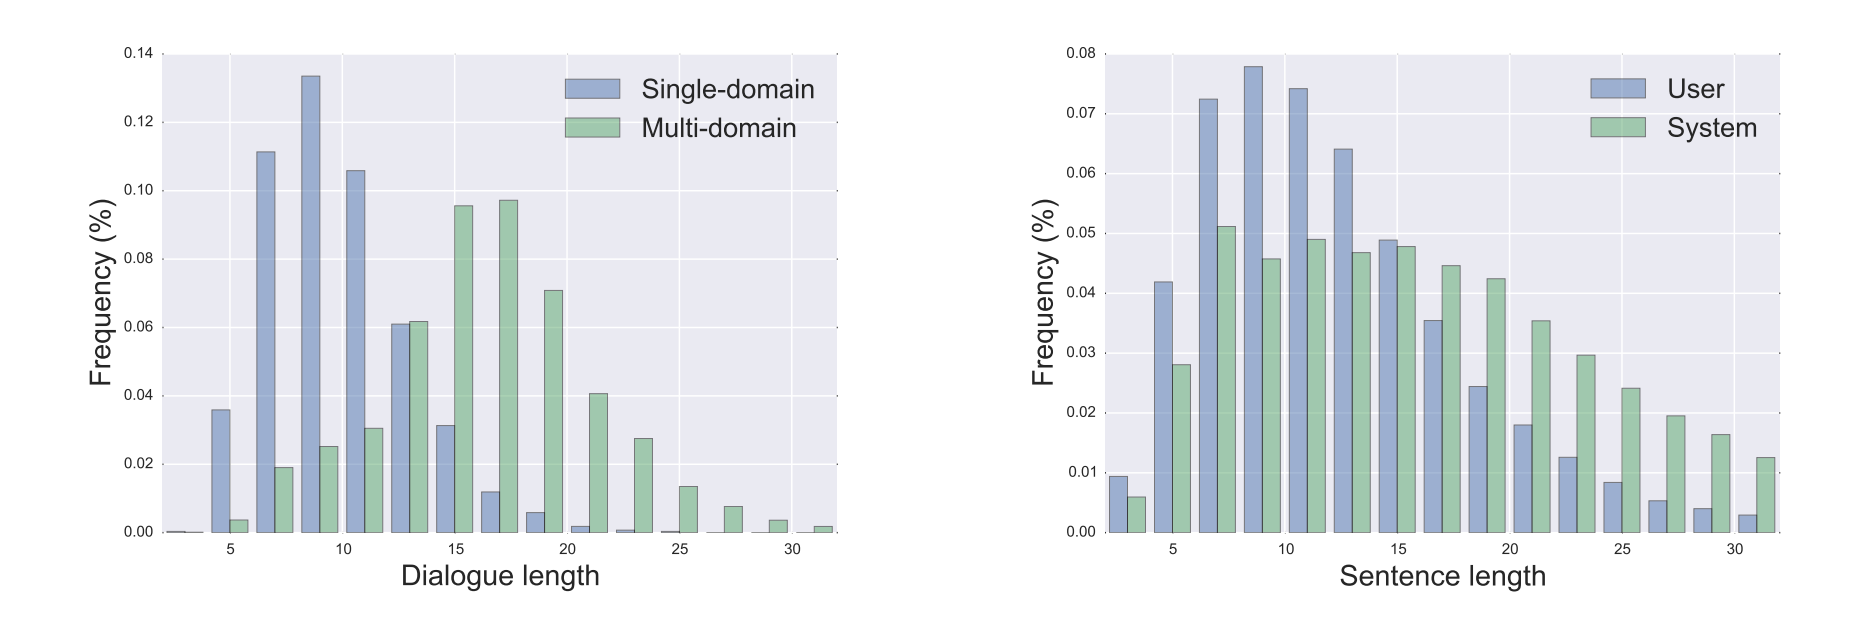
\includegraphics[width=\textwidth]{./images/multiwoz-stats.png}
  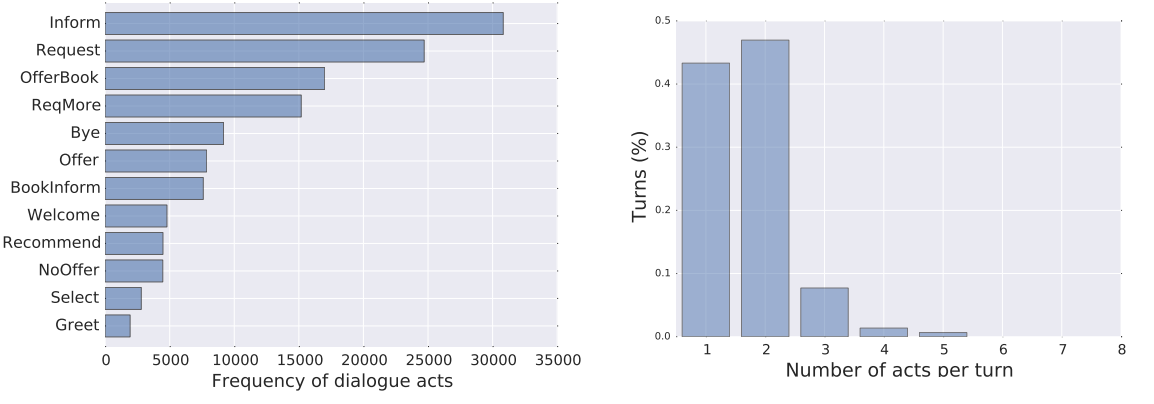
\includegraphics[width=\textwidth]{./images/acts.png}
\end{figure*}


\begin{table*}[!ht]
  \caption{Summary of the MultiWOZ dataset}
  \centering
  \begin{tabularx}{\textwidth}{lp{10cm}lll}
    \toprule
    \multicolumn{1}{l}{Domain} & \multicolumn{1}{c}{Slots}                                                    & \multicolumn{3}{c}{Split}              \\
    \cmidrule(l){3-5}
                               &                                                                              & Train                     & Dev & Test \\
    \midrule
    Attraction                 & area, name, type                                                             & 3,381                     & 416 & 394  \\
    Hotel                      & area, bookday, num\_people, internet, name, parking, pricerange, stars, type & 3,103                     & 484 & 494  \\
    Restaurant                 & area, bookday, num\_people, book\_time, pricerange                           & 2,717                     & 401 & 395  \\
    Taxi                       & arriveby, departure, destination, leaveat                                    & 3,813                     & 438 & 437  \\
    Train                      & arriveby, bookpeople, day, departure, destination, leaveat                   & 1,654                     & 207 & 195  \\
    \bottomrule
  \end{tabularx}
\end{table*}

\section{Dataset}

MultiWOZ is a large fully-labeled collection of human-human written conversations spanning over multiple domains and topics \cite{Budzianowski2018MultiWOZA}. It has 3,406 single-domain dialogues and 7,032 multi-domain dialogues consisting of 2-5 domains. There are on average 13.5 \textit{turns per dialogue}. The average sentence lengths are 11.75 and 15.12 for users and wizards respectively. Each dialogue consists of a pre-defined user goal, and multiple user and system utterances as well as an implicit belief state. The data spans 7 domains --- \texttt{Restaurant, Hotel, Taxi, Train, Attraction, Hospital, Police}.

MultiWOZ 2.1 is a recent effort to address the shortcomings of  \texttt{v2.0}. The original utterances were re-annotated completely to account for the noisy annotations. Additionally, the user dialog acts were annotated, which were missing from the original dataset. The correction impacted 32\% of state annotations across 40\% of dialogue turns.

\begin{figure*}[!ht]
  \centering
  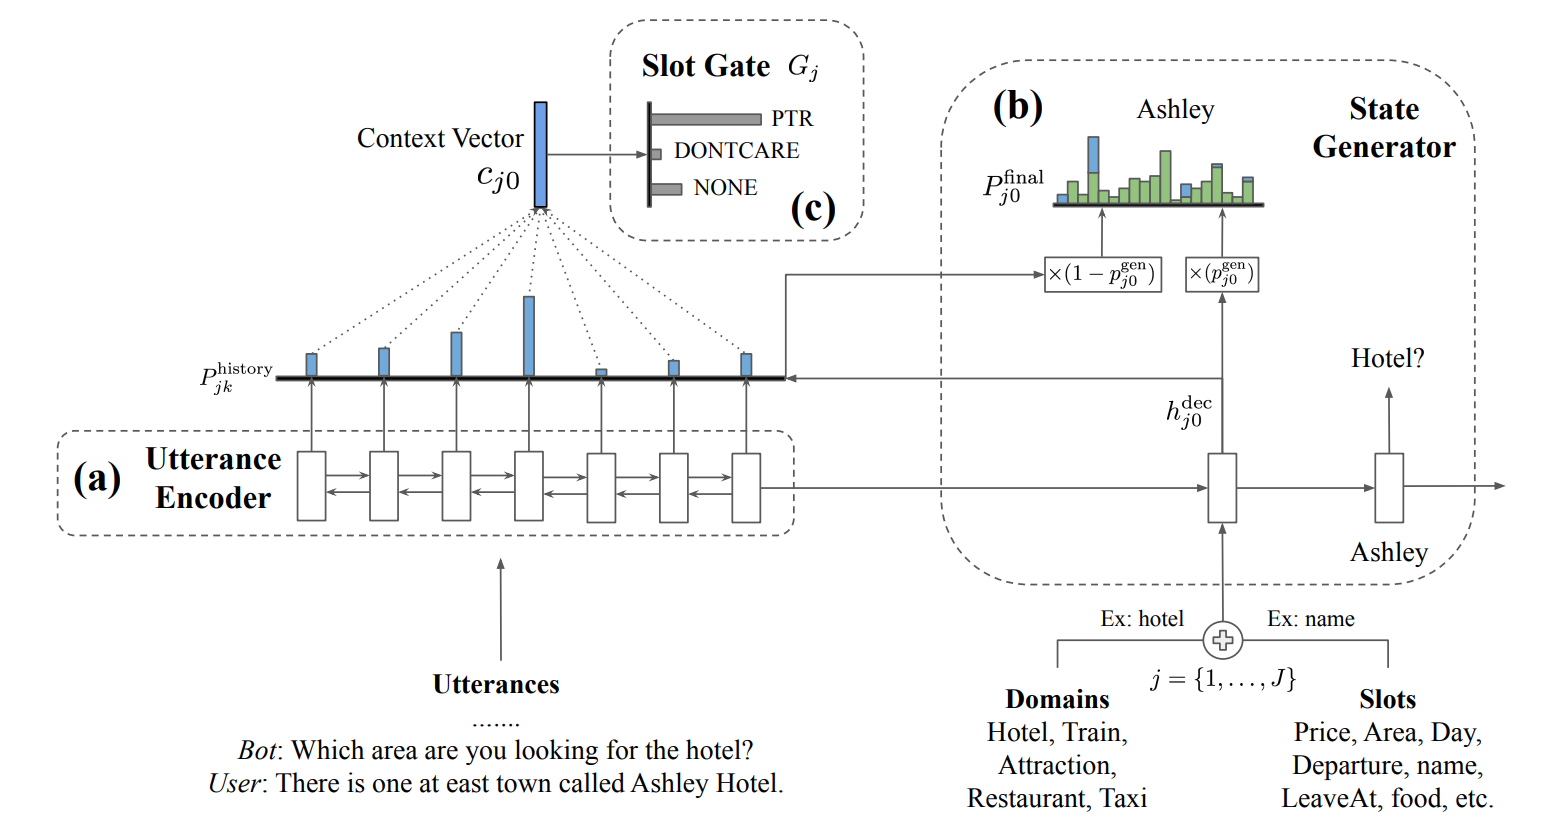
\includegraphics[width=\textwidth]{./images/trade.png}
  \caption{TRADE model architecture. We modify the utterance encoder component}
\end{figure*}

\subsection{Data Collection Process}

Data is collected by simulating tourist desk information agents and users by Mechanical Turkers. To facilitate data collection, \cite{Budzianowski2018MultiWOZA} provide an easy-to-operate interface. An intial set of trials were used to identify a set of workers that perform annotation well. These workers were then asked to annotate the real dialogues. A large number of workers are used to facilitate diversity.

\medskip \noindent \textbf{User side}: A goal is conveyed to a user and the various constraints are communicated gradually to avoid information overload and mimic a natural conversation.

\medskip \noindent \textbf{System side}: The system agent or \textit {wizard} is asked to perform a role of a clerk and provide information to the user. They have access to a fixed ontology for reference. The wizard either gives the result of the user supplied query or requests for more information necessary for the search query. The wizards communicate via a web form, which is also used to implicitly track the belief state of the dialogue.

\bigskip \noindent The dataset comes with a pre-defined train/test/dev split of \texttt{8k/1k/1k} dialogues, for easier reproducibility, and we continue to use the same split in all our experiments. Since, some of the dialogues ended up with the user goal unmet; the validation and test sets only contain dialogues that were successful.


\subsection{Data Pre-processing}

We perform the following pre-processing steps on the data. We \textit{delexicalize} the data using the scripts provided in the MultiWOZ repository. The entities mentioned in the dialogue acts, such as \textit{restaurant-name}, are encoded as one-hot vectors. We generate a vocabulary from the input and a mapping of index to words is generated for easier embedding. Further, the dialogues are divided into train/val/test split and the text is lowercased. Further, the \textit{hospital} and \textit{police} domain are removed from the dataset as they are only present in the train, and have few dialogues.

\begin{table*}[!htbp]
  \caption{Experimental Results}
  \centering
  \begin{tabularx}{0.8 \textwidth}{Xccc}
    \toprule
    Model              & \multicolumn{3}{c}{Metrics}                         \\
    \cmidrule{2-4}
                       & Joint Accuracy              & Slot Accuracy & F1    \\
    \midrule
    Trade DST*         & 0.480                       & 0.969         & 0.87  \\
    NADST              & 0.469                       & 0.971         & 0.880 \\
    NADST + ConceptNet & 0.460                       & 0.966         & 0.835 \\
    NADST + GloVE      & 0.477                       & 0.992         & 0.890 \\
    \bottomrule
  \end{tabularx}
  \label{results}
\end{table*}

\section{Approach}

Let $X = \{(U_t, R_t)\}$ be the set of user utterances and system utterances up to turn $t$. We encode the dialog history using a bi-directional gated recurrent units (GRU) to get the dialogue history. Encoding the dialogue history enables us to handle multi-turn dialogue.

\textit{ConceptNet} is a Knowledge Base consisting of 8m facts and relations \cite{Liu2004ConceptNetA}. ConceptNet Numberbatch are vectors built using an ensemble that combines data from ConceptNet, word2vec, GloVe, and OpenSubtitles 2016, using a variation of a method known as \textit{retrofitting} \cite{Speer2016ConceptNet5A}. The embedding of a node are created to minimize the vectors's euclidean distance to its graph neighbours as well as to the distance of equivalent pre-trained embeddings such as GloVE \cite{Pennington2014GloveGV}, fastText. The resulting embeddings capture the graph knowledge.

\subsection{Metrics}

For our experiments, we use the following metrics,

\begin{enumerate}
  \item \textbf{Joint Accuracy}: The joint accuracy is the ratio of dialogue turns where \textbf{all} slots are classified correctly. This metric gives us a good estimate of the robustness of the overall system.
  \item \textbf{Slot Accuracy}: This is the ratio of correctly classified slots over all dialogue turns.
  \item \textbf{F1 score}: The F1 score computed over all the slots.
\end{enumerate}

\section{Experiments}

The models are built in PyTorch 1.5. We use the \textit{Adam} optimizer with $betas = (0.9, 0.98)$ and a learning rate $\alpha = 0.001$. The dropout is set to $dropout = 0.2$. Further we use a batch size of $32$ in all our experiments. The model is trained on a TitanX 12GB gpu for 30 epochs or until convergence. We use a a train/dev/test split of \texttt{8k/1k/1k} examples, divided according to class proportions. Additionally, we leave out the \textit{hospital} and \textit{police} domain, since they constitute $\le 10\%$ of the train data and are absent from the test and dev set.

For our baseline, we use the TradeDST model architecture, consisting of an utterance decoder, slot gate and state generator; described previously. The utterance encoder uses an embedding layer of $d = 256$, initialized uniformaly at random, which is also jointly trained. The TradeDST model is trained on MultiWOZ 2.0 dataset, an earlier version compared to our dataset. The annotations in MultiWOZ 2 was dominated by \texttt{none} class. *Models trained on this dataset were biased towards predicting \texttt{none} class, resulting in a higher score (as seen from the baseline TradeDST model). This imbalance was corrected in MultiWOZ 2.1, which makes it more challenging. The results are summarized in Table \ref{results}.

Next, we initalize the embedding layer with GLoVe CommonCrawl embeddings $300$-d. These embeddings are trained on 42B tokens with approximately 1.9M vocabulary size. We filter the vocabulary based on our target dataset. The model is trained with the same hyperparamters as our baseline model. We see that there is an improvement in the model performance across all the metrics.

Finally, we induce external knowledge into the utterance encoder through the ConceptNet numberbatch embeddings. However, there is no significant improvement over the baseline, which we hypothesize could be due to 2 reasons. (1) ConceptNet is a huge knowledge graph with over 8m entities and relations. The majority of these relations are unhelpful for our dialogue system. (2) ConceptNet is still vastly incomplete for it to be useful.

\section{Conclusion}

Task-oriented dialogue systems continue to be widely used. A dialogue state tracker keeps track of the dialogue state at each turn. In this paper, we evalutate the performance of various word embeddings in the utterance encoder module, in the scope of multi-domain dialogue state tracking. We see from our experiments that using pre-trained embeddings such as GloVE improve the performance of the model in zero-shot learning in terms of the slot extraction. However, we also notice incorporating Knowledge Base embeddings in the model doesn't help and an alternative is needed to induce external knowledge.

\nocite{*}
\bibliography{references}

\end{document}
